\section{Event Preselection and Reconstruction}
To suppress SM backgrounds while keeping the signal events at high efficiency, event selection criteria are made to select interesting events from the datasets. Preselection is first performed and works as control region to help optimize the background modeling. Afterwards, further selections are made as signal region selections, which will be discussed in Section~\ref{sec:selection_sr}.

\subsection{Lepton Selection}
Electrons and muons are selected from both single lepton datasets and the MC simulation samples, and paired to be reconstructed as a Z boson. The detail selections are described below in addition to the single lepton HLT requirements.
\subsubsection{Electron Pair Selection}
Both electrons in an selected electron pair are are required to pass the Egamma loose cut-based Identification and Isolation as described in Section~\ref{sec:ob_eidiso} to be regarded as a well-identified electron. Besides, more criteria are required on the $p_T$ and $\eta$ values of the leading and subleading electrons in the pair, as listed below.
\begin{enumerate}
\item Leading Electron: $p_T >120 GeV$, $|\eta|<2.5$
\item Subleading Electron: $p_T >35 GeV$, $|\eta|<2.5$
\end{enumerate}

The restriction on their $|\eta|$ value is due to the design of the ECAL detector. And for the leading electron, only those with $p_T$ beyond 120 GeV will be kept, because of the single electron HLT (\texttt{HLT\_Ele115\_CaloIdVT\_GsfTrkIdT}) we use has a threshold at 115 GeV. More discussion can be found in Section~\ref{sec:bkg_trig}.

\subsubsection{Muon Pair Selection}\label{sec:muonselection}
Two Muon Identifications are involved in the muon pair selection as described in Section~\ref{sec:ob_midiso}, to optimize the muon pair selection efficiency. Various combination of muon IDs are considered, and Figure~\ref{fig:sel_mumueff} shows the muon pair efficiencies for different muon ID combinations, versus $\Delta R$ between the two muons in the pair, and the $p_T$ of the muon pair.

\begin{figure}[htbp]
\begin{center}
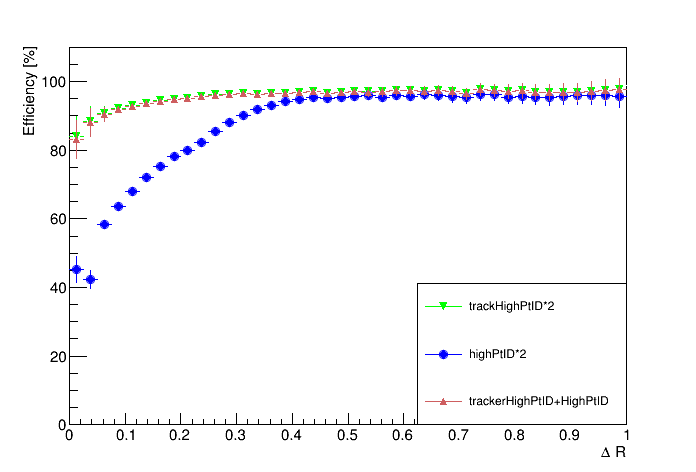
\includegraphics[width=0.9\linewidth]{figures/sel_mudreff.png}
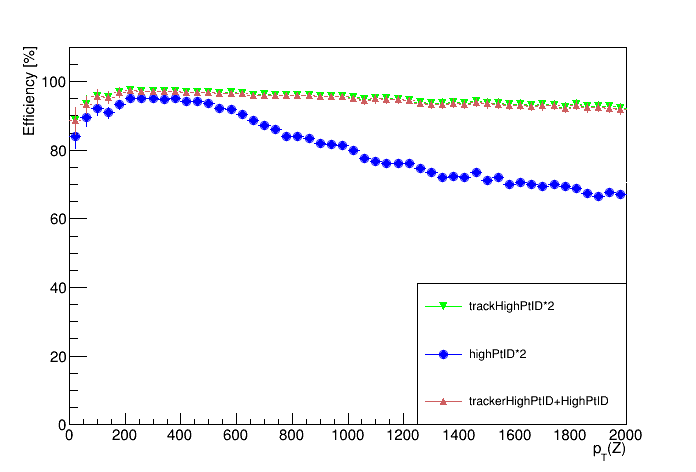
\includegraphics[width=0.9\linewidth]{figures/sel_muzpteff.png}
\caption{Efficiency comparison among various muon ID combinations, versus $\Delta R$ between the muons (upper) and $p_T$ of the muon pair (lower).}
\label{fig:sel_mumueff}
\end{center}
\end{figure}

\vspace{0.3cm}
The efficiency profiles are obtained from the signal MC samples generated by Madgraph, and generator level information is used to judge if a reconstructed muon is a true muon or not. The two efficiency plots are consistent considering the fact that the $\Delta R$ between the muons are likely to be smaller in a pair with higher $p_T$. From the plot, one can see huge sacrifice in efficiency by requiring both muons to pass the High $p_T$ ID, because the resolution of the muon system is not high enough to distinguish such two adjacent muons and reconstruct them as separated tracks. However, the other two ID combination, two Tracker High $p_T$ ID combination and Tracker High $p_T$ ID $+$ High $p_T$ ID combination, show very similar efficiency performance, which is stably high in the high $p_T$ region. Considering that the High $p_T$ ID is a tighter identification compared to the tracker High $p_T$ ID, the Tracker High $p_T$ ID $+$ High $p_T$ ID combination is used as the muon identification in this analysis, to secure high selection efficiency as well as good muon identification quality. In addition to the muon identification, $relIso_{tk}<0.1$ is also required for each of the muons in the pair as isolation selection, as described in~\ref{sec:ob_midiso}.

\vspace{0.3cm}
Like the electron selection, more criteria on the muons' $p_T$ and $\eta$ values are listed below:
\begin{enumerate}
\item Leading Muon: $p_T >60 GeV$, $|\eta|<2.4$
\item Subleading Muon: $p_T >20 GeV$, $|\eta|<2.4$
\end{enumerate}

The restriction on their $|\eta|$ value is due to the design of muon system detector. For the leading muon, $p_T >60 GeV$ is required considering the single muon HLTs (\texttt{HLT\_Mu50} and \texttt{HLT\_TkMu50}) have thresholds at 50 GeV.

\subsection{Leptonic Z Boson Reconstruction}
A selected lepton pair can either be an electron pair or a muon pair, and the two leptons are required to have opposite charge. In one event, more than one such lepton pairs can exist, and in this case, the best lepton pair will be selected. The the best pair selection is based on the invariant mass of the lepton pair: only the lepton pair with the invariant mass closest to the true Z boson mass (91.1876 GeV) will be selected among all the lepton pairs in an event. A Z mass window is set between 70 GeV and 110 GeV, so only events with lepton pair's invariant mass within the Z mass window are kept.

\vspace{0.3cm}
To suppress the low energy backgrounds, $p_T ^Z > 50GeV$ is required for the pre-selection.


\subsection{MET Filters}\label{sec:metfilter}
Based on the recommendation by the JetMET group, MET filters are applied to ensure the quality of the MET reconstruction, for both Monte Carlo samples and data. The MET filters are listed below:
\begin{itemize}
\item \texttt{Flag\_EcalDeadCellTriggerPrimitiveFilter}
\item \texttt{Flag\_HBHENoiseIsoFilter}
\item \texttt{Flag\_goodVertices}
\item \texttt{Flag\_HBHENoiseFilter}
\item \texttt{Flag\_globalTightHalo2016Filter}
\item \texttt{Flag\_eeBadScFilter}
\item \texttt{Flag\_BadPFMuonFilter}
\item \texttt{Flag\_BadChargedCandidateFilter}
\item \texttt{Flag\_noBadMuons}
\end{itemize} 

More information about MET filters can be found [\href{https://twiki.cern.ch/twiki/bin/viewauth/CMS/MissingETOptionalFiltersRun2?rev=103}{here}].

\section{Signal Region}\label{sec:selection_sr}
To further suppress the background and improve the statistical significance of the search, a signal region is defined. On top of the pre-selection, further selection on the lepton pair $p_T$ and $p_T ^{miss}$ are made as following: $p_T ^Z > 100GeV$ and $p_T ^{miss} > 50GeV$, to match the signature of the two boosted Z bosons of the analysis. 

\vspace{0.3cm}
Additionally, because in the signal model the two Z bosons come from the decay of a heavy resonance, and thus are mostly back to back, the variable $|\Delta \Phi (p_T ^Z ,p_T ^{miss})|$, which shows the angle difference in the XY plane between $p_T ^Z$ and $p_T ^{miss}$, is used to help separating the signal and background, especailly $Z+jets$ events. The signal events tend to have large $|\Delta \Phi (p_T ^Z ,p_T ^{miss})|$ value, while for the $Z+jets$ events, $|\Delta \Phi (p_T ^Z ,p_T ^{miss})|$ should be generally flat, since the $p_T ^{miss}$ is instrumental and does not have a preferred direction with respect to the leptonic Z boson. Therefore, $|\Delta \Phi (p_T ^Z ,p_T ^{miss})|>0.5$ is applied in the signal region. 

\vspace{0.3cm}
To sum up, the selection critieria in the signal region are shown as below:
\begin{enumerate}
\item Trigger: single muon and single electron triggers as documented in Section~\ref{sec:samples_hlt}
\item Lepton ID and ISO:
  \subitem Muons: Tracker High $p_T$ ID $+$ High $p_T$ ID combination in a muon pair, 
  both muons are also required to pass tracker ISO
  \subitem Electrons: both electrons pass Loose Electron ID and corresponding PF Isolation
\item Lepton acceptance cuts:
  \subitem Muons: Leading  $p_T > 60 GeV$, subleading $p_T > 20 GeV$, both muons in $|\eta| < 2.4$
  \subitem Electrons: Leading $p_T >120 GeV$, subleading $p_T >35 GeV$, both electrons in $|\eta|<2.5$
\item Dilepton pair selection: A pair of same flavor opposite sign
  leptons with a closest invariant mass to the true Z boson mass
\item Z mass window:   $70 < |M_{ll}| < 110 GeV$
\item Z boson: $p_T >100 GeV$
\item Missing $p_T$: $p_T ^{miss} > 50GeV$
\item $|\Delta \Phi (p_T ^Z ,p_T ^{miss})|>0.5$
\end{enumerate}

